\clearpage

\section{Pseudo-Goldstone gap: derivation and
calculation}\label{sec-nbcp-gap-appendix}

The spin-orbit-coupling-induced pseudo-Goldstone gap in the
three-sublattice Y and V states depends on two ingredients: the quantum
energy curvature along a classical equal-energy orbit and the classical
response conjugate to that orbit. For the nearest-neighbor model
considered here, the soft coordinate is a common laboratory-\(z\)
rotation. Its relaxed conjugate motion is a nonuniform change of the
polar angles, determined by the longitudinal susceptibility. This
distinction explains why a uniform polar-angle increment in the archived
calculation does not reproduce the leading-order gap.

\begin{tcolorbox}[colback=NotePale,colframe=NoteAccent,boxrule=0pt,leftrule=2pt,arc=0pt]

\textbf{Leading-order relation}

\begin{equation}\phantomsection\label{eq-lswt-yv-pg-gap}{
C_\phi=\left.\frac{\partial^2 e_{\rm sw}}{\partial\phi^2}\right|_{\phi_*},
\qquad
\Delta_{\rm PG}=\hbar\omega_{\rm PG}
=\sqrt{\frac{C_\phi}{\chi_z}}.
}\end{equation}

Here \(e_{\rm sw}\) is the energy per physical spin, \(\phi_*\) is its
selected angular minimum, and \(\chi_z=\partial m_z/\partial h\) is
evaluated along the relaxed classical branch. The reduction requires a
stable background and finite classical stiffness in the other uniform
modes.

\end{tcolorbox}

\subsection*{Conventions at a glance}\label{conventions-at-a-glance}
\addcontentsline{toc}{subsection}{Conventions at a glance}

\begin{longtable}[]{@{}
  >{\raggedright\arraybackslash}p{(\linewidth - 2\tabcolsep) * \real{0.5000}}
  >{\raggedright\arraybackslash}p{(\linewidth - 2\tabcolsep) * \real{0.5000}}@{}}
\toprule\noalign{}
\begin{minipage}[b]{\linewidth}\raggedright
Quantity
\end{minipage} & \begin{minipage}[b]{\linewidth}\raggedright
Meaning and normalization
\end{minipage} \\
\midrule\noalign{}
\endfirsthead
\toprule\noalign{}
\begin{minipage}[b]{\linewidth}\raggedright
Quantity
\end{minipage} & \begin{minipage}[b]{\linewidth}\raggedright
Meaning and normalization
\end{minipage} \\
\midrule\noalign{}
\endhead
\bottomrule\noalign{}
\caption{Coordinates and normalizations used in the pseudo-Goldstone calculation.}\label{tab-nbcp-a-pseudo-goldstone-gap-1}\\
\endlastfoot
\(\phi\), \(q=\phi-\phi_*\) & Common physical rotation about laboratory
\(z\); angles in radians \\
\(\boldsymbol\vartheta\) & Signed polar-angle chart for the three
sublattices \\
\(m_z=(S/3)\sum_\alpha\cos\vartheta_\alpha\) & Magnetization per
physical spin, in dimensionless spin units \\
\(h=g_z\mu_B B\) & Zeeman energy in \(-h\sum_i S_i^z\); measured in
meV \\
\(A\), \(\mathbf w\) & Polar Hessian per three-spin cell;
\(w_\alpha=-S\sin\vartheta_\alpha\) \\
\(C_\phi\), \(\chi_z\) & Angular energy curvature per spin;
susceptibility in meV\(^{-1}\) \\
\end{longtable}

The symbols \(e\), \(A\), and the sublattice labels \(\alpha=A,B,C\)
retain the conventions of the comparison data. In particular, \(A\) is a
classical polar Hessian, not the normal block of a bosonic Hamiltonian.
No extra \(g_z\mu_B\) or spin-length factor is appended to the gap.

\textbf{Reading route.} The classical orbit is specified first; the
Berry term and constrained relaxation then determine its canonical
partner. The Y and V specializations precede the numerical comparison.
Implementation findings, convergence tables, and reproduction details
are collected in Section~\ref{sec-nbcp-verification-appendix} and the
linked physics-to-code review record.

\clearpage

\subsection{Model and equal-energy orbit}\label{sec-orbit}

The target is the spin-orbit-coupling (SOC) induced gap of the common
global-\(z\) orbit in Park et
al.~(2026)~\cite{park2026}. The internal, nonuniform zero-field XXZ mode discussed by
Lin and Shi (2025)~\cite{lin2025} is a
different excitation. That distinction is essential when choosing the
deformation used to calculate the curvature.

Only nearest-neighbor bonds are included, with \(S=1/2\), \(J=0.075\)
meV, \(J_z=0.125\) meV and \(T=0\). The representative fields are
\(B=0.2\) T in Y and \(B=1.4\) T in V, with \(g_z=4.645\). The two SOC
coefficients are denoted by \(J_{PD}\) and \(J_\Gamma\).

\subsubsection{Common laboratory
rotation}\label{common-laboratory-rotation}

\begin{equation}\phantomsection\label{eq-lswt-yv-pg-orbit}{
\mathbf S_\alpha(\phi)=R_z(\phi)\mathbf S_\alpha(0)
=S\begin{pmatrix}
\sin\vartheta_\alpha\cos\phi\\
\sin\vartheta_\alpha\sin\phi\\
\cos\vartheta_\alpha
\end{pmatrix},\qquad \alpha=A,B,C.
}\end{equation}

The same lab-frame rotation acts on all three spins. In the
signed-polar-angle chart used here, opposite transverse directions are
represented by opposite signs of \(\vartheta\), with a common azimuth.
This is a physical spin rotation, not a rotation of a local transverse
basis about a fixed spin.

For the three nearest-neighbor bond orientations,
\(\sum_d J_d=3\operatorname{diag}(J,J,J_z)\). Each A-B, B-C and C-A pair
has all three orientations. Thus PD and Gamma cancel in the classical
three-sublattice energy for every \(\phi\), while they remain in the
finite-momentum spin-wave Hamiltonian. This is an accidental degeneracy
when SOC is nonzero. At zero SOC the same orbit is an exact U(1)
symmetry and this particular gap is exactly zero.

Equal energy on this restricted manifold does not prove a global
classical minimum; the finite-momentum Hessians are separately checked
for stability. Unstable angular backgrounds are rejected rather than
shifted.

\begin{figure}[htbp]

\centering{

\nbcpbounded{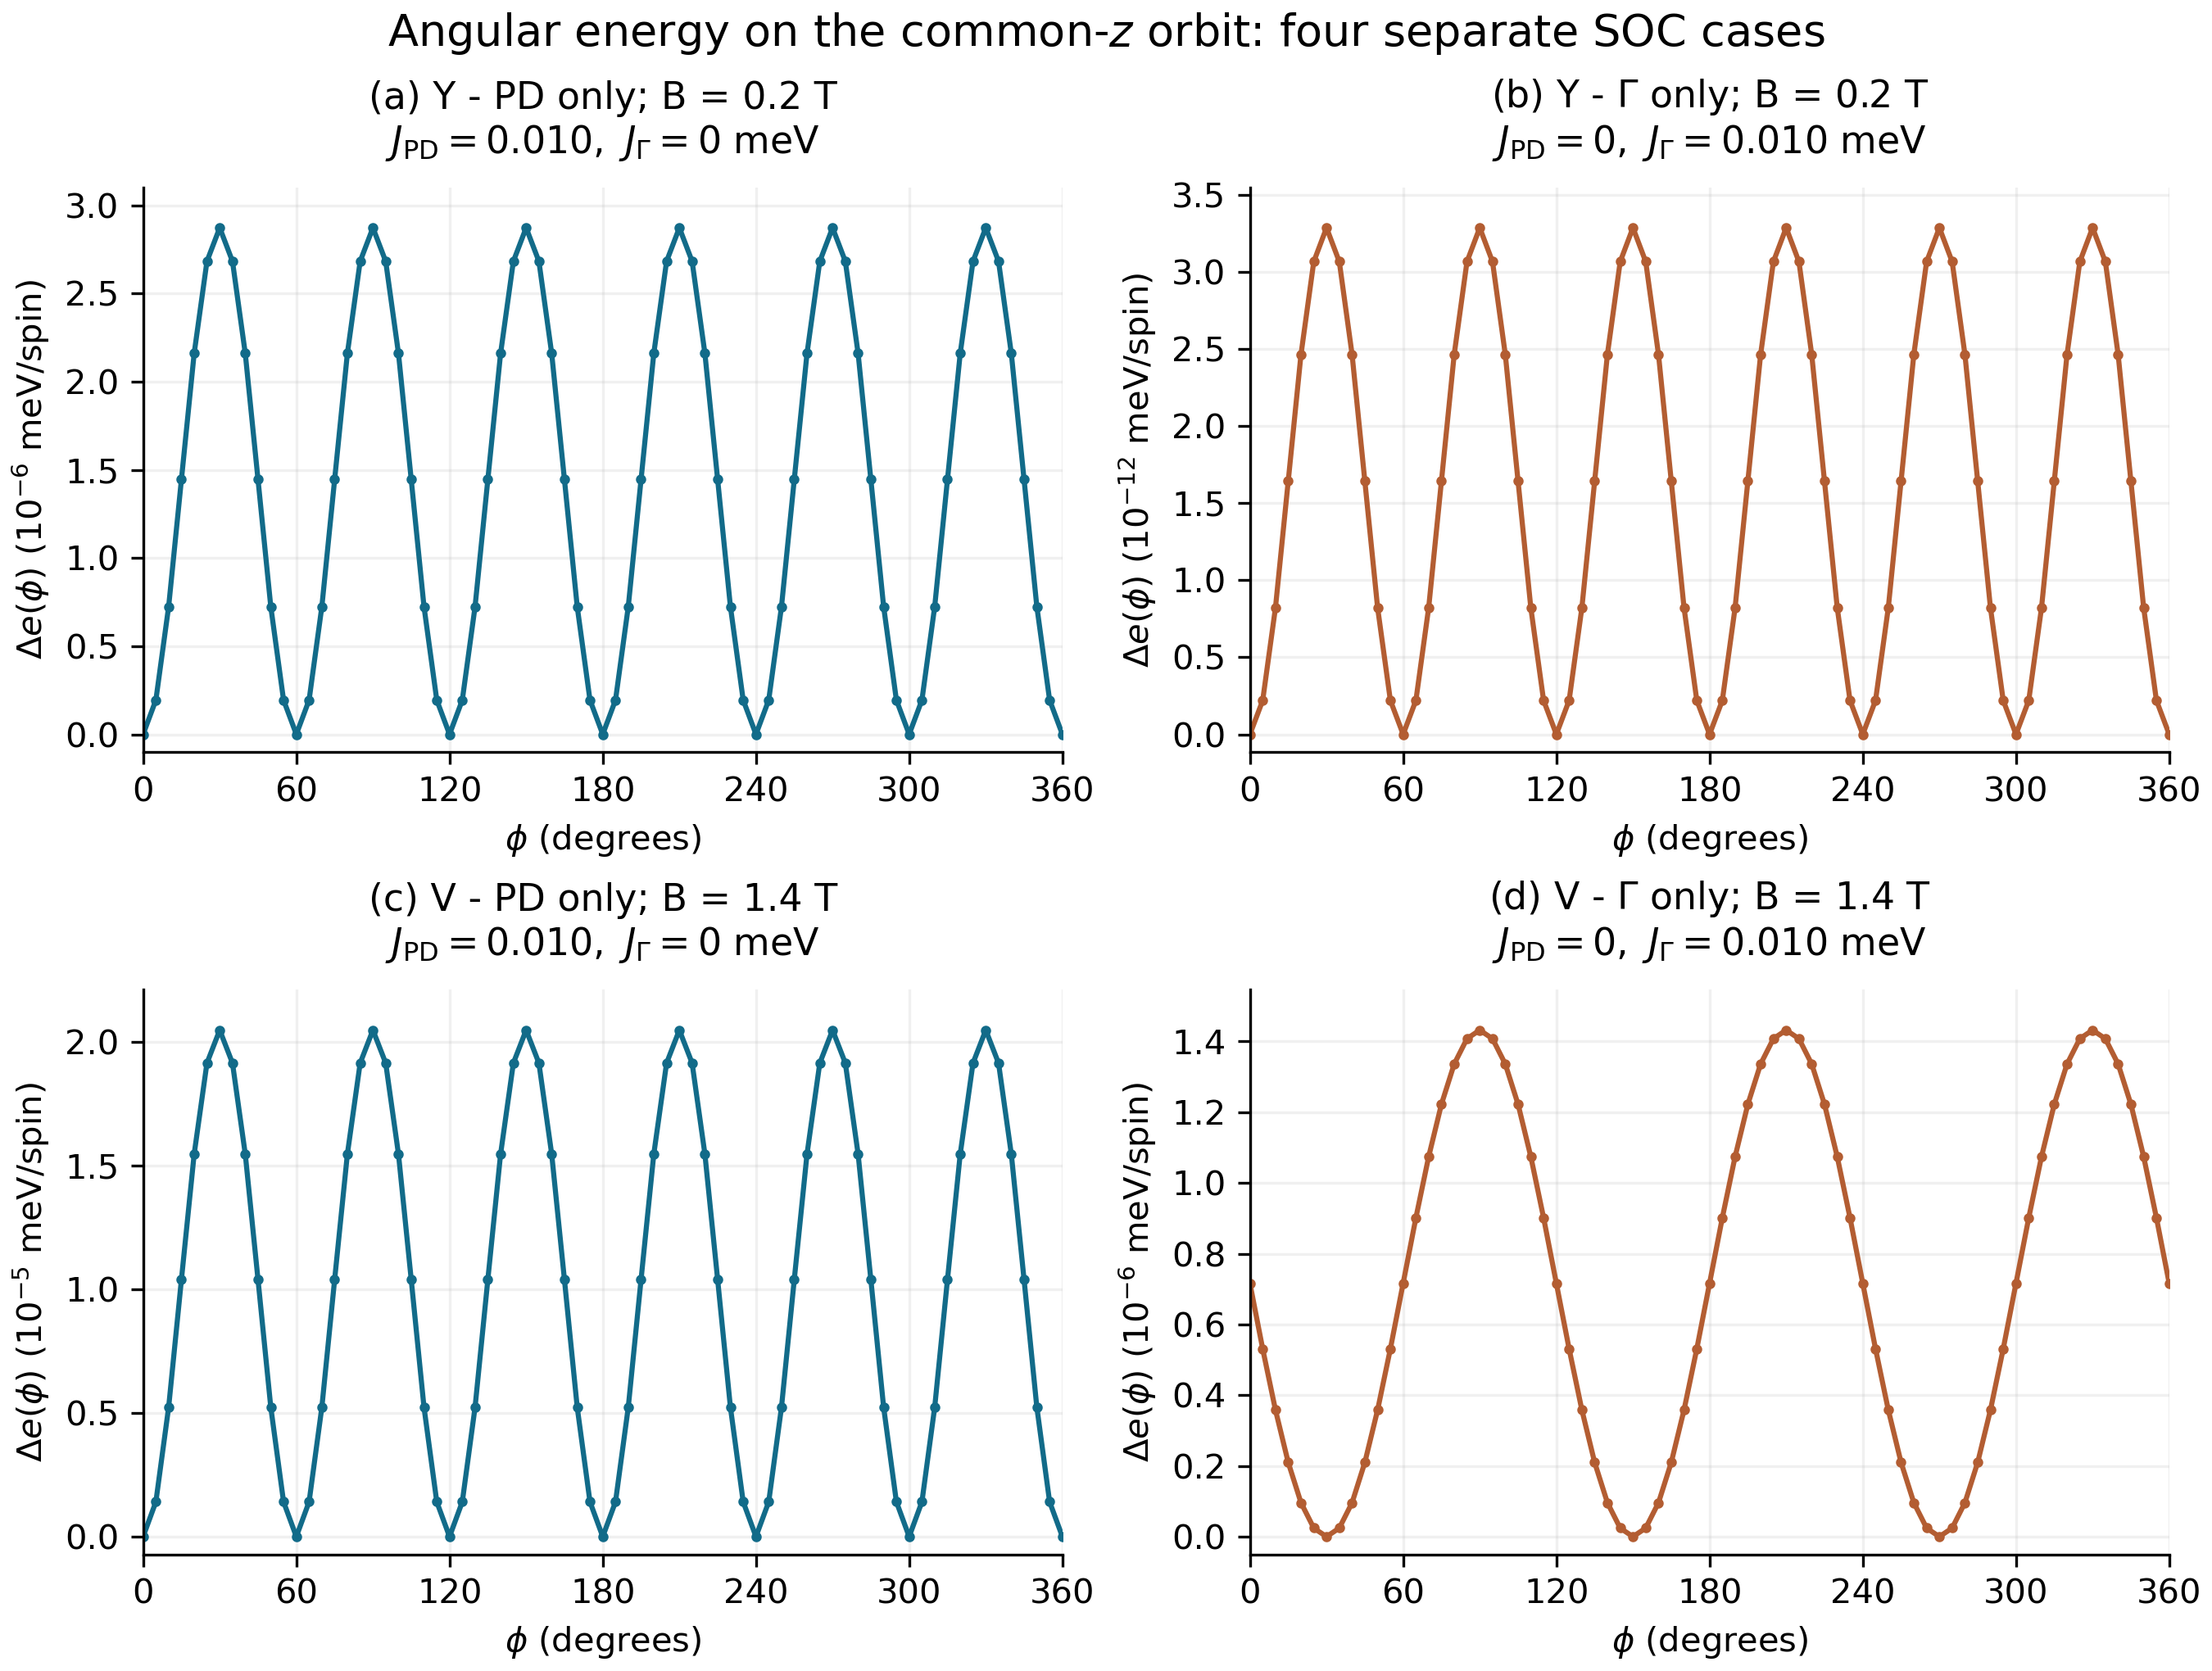
\includegraphics[keepaspectratio]{../../data-space/verification/260917-clock-matching/yv-angular-energy-four-cases.png}}

}

\caption{\label{fig-yv-orbit}Angular energy for four separately
activated SOC cases: Y--PD, Y--Gamma, V--PD and V--Gamma. The active
coupling is 0.010 meV and the other is zero; Y uses B=0.2 T and V uses
B=1.4 T. Each panel shows the current-Hamiltonian semiclassical energy
difference per spin, evaluated from the zero-point component because the
classical orbit energy is constant. The vertical axes use explicitly
different absolute scales. Points are the saved 72-angle samples at base
mesh N=48; the final point repeats the first at 360 degrees. No harmonic
fit or new diagonalization is used.}

\end{figure}%

\subsection{Canonical response and the gap}\label{sec-canonical}

The curvature relation is specialized here to the common
laboratory-\(z\) orbit. The following Y/V expressions are the derivation
used in this comparison, rather than formulas quoted directly from the
cited papers.

\subsubsection{Berry term and
magnetization}\label{berry-term-and-magnetization}

Write \(q=\phi-\phi_*\) and let \(\mathbf x=\delta\boldsymbol\vartheta\)
denote polar displacements from a stationary coplanar state. The spin
Berry term, in a gauge differing from other common gauges by a total
derivative, is \(L_B=\hbar S\sum_i\cos\vartheta_i\,\dot\phi_i\). A
common azimuth therefore couples to the total z magnetization. Per
physical spin,

\begin{equation}\phantomsection\label{eq-lswt-yv-pg-berry}{
\ell_B=\hbar m_z\dot q,
\qquad
p\equiv\delta m_z=\frac{\mathbf w^{\mathsf T}\mathbf x}{3},
\qquad
w_\alpha=-S\sin\vartheta_\alpha.
}\end{equation}

The constant equilibrium term \(\hbar m_{z,0}\dot q\) does not affect
the local equations of motion. The physical spin tangent of the global-z
orbit is
\(\partial_q\mathbf S_\alpha=S\sin\vartheta_\alpha\,\mathbf e_{\phi,\alpha}\).
Thus a common azimuth does not produce equal local transverse
displacements. In the Y state the axial spin has zero tangent on this
orbit. This statement remains regular in Cartesian tangent coordinates
even though its individual azimuth is undefined at the pole.

\subsubsection{Relaxation at fixed
magnetization}\label{relaxation-at-fixed-magnetization}

For the common-azimuth states, the classical energy per magnetic cell is

\begin{equation}\phantomsection\label{eq-lswt-yv-pg-classical-energy}{
E_{\rm cl}^{\rm cell}
=3S^2\sum_{(\alpha\beta)=(AB),(BC),(CA)}
\left[J\sin\vartheta_\alpha\sin\vartheta_\beta
+J_z\cos\vartheta_\alpha\cos\vartheta_\beta\right]
-hS\sum_\alpha\cos\vartheta_\alpha.
}\end{equation}

The SOC cancellation on this uniform three-sublattice manifold is why
the same expression supplies the classical hard stiffness. Assume that
\(A\) is positive definite and that the common-z direction is the only
soft uniform mode. At fixed \(p=\delta m_z\), the classical energy cost
is obtained by minimizing \(\mathbf x^{\mathsf T}A\mathbf x/6\) subject
to \(\mathbf w^{\mathsf T}\mathbf x=3p\). The stationary solution is

\begin{equation}\phantomsection\label{eq-lswt-yv-pg-fixed-magnetization}{
\mathbf x_*(p)
=\frac{3A^{-1}\mathbf w}{\mathbf w^{\mathsf T}A^{-1}\mathbf w}\,p,
\qquad
\delta e_{\rm cl,min}=
\frac{3p^2}{2\mathbf w^{\mathsf T}A^{-1}\mathbf w}
=\frac{p^2}{2\chi_z}.
}\end{equation}

The same response follows without a dynamical assumption by
differentiating the classical stationarity equation with respect to the
Zeeman energy \(h\):

\begin{equation}\phantomsection\label{eq-lswt-yv-pg-susceptibility}{
A\frac{d\boldsymbol\vartheta}{dh}=\mathbf w,
\qquad
\chi_z=\frac{1}{3}\mathbf w^{\mathsf T}A^{-1}\mathbf w,
\qquad
\frac{d\boldsymbol\vartheta}{dm_z}=\frac{A^{-1}\mathbf w}{\chi_z}.
}\end{equation}

The quadratic effective energy per spin near the selected angle is

\[
\delta e=\frac{(\delta m_z)^2}{2\chi_z}
+\frac{C_\phi}{2}(\delta\phi)^2.
\]

With the Berry term \(\hbar\,\delta m_z\,\partial_t\delta\phi\), the
linear equations give
\(\hbar^2\partial_t^2\delta\phi=-(C_\phi/\chi_z)\delta\phi\), yielding
the gap in Eq.~\ref{eq-lswt-yv-pg-gap}. The total Lagrangian contains
the common factor \(N_{\rm site}\), which cancels from the equations of
motion.

\subsubsection{Trial directions and their
stiffness}\label{trial-directions-and-their-stiffness}

For \(\mathbf x=\mathbf u\,\xi\), with a fixed trial direction
\(\mathbf u\), define

\begin{equation}\phantomsection\label{eq-lswt-yv-pg-trial-coordinates}{
b_{\mathbf u}=\frac{\mathbf w^{\mathsf T}\mathbf u}{3},
\qquad
\kappa_{\mathbf u}=\frac{\mathbf u^{\mathsf T}A\mathbf u}{3}.
}\end{equation}

Here \(A\) is the classical polar Hessian per three-spin magnetic cell,
not a particle block of the spin-wave matrix. The restricted Berry term
is \(\hbar b_{\mathbf u}\xi\dot q\). If \(b_{\mathbf u}=0\), these two
coordinates do not form a canonical pair. If it is nonzero,
\(p_{\mathbf u}=b_{\mathbf u}\xi\) is a canonical momentum on this
restricted surface, whose trial gap is

\begin{equation}\phantomsection\label{eq-lswt-yv-pg-trial-gap}{
\Delta_{\mathbf u}^{\,2}
=\frac{C_\phi\kappa_{\mathbf u}}{b_{\mathbf u}^{2}}.
}\end{equation}

This is a prediction of the restricted two-coordinate model, not
automatically a normal-mode frequency of the full spin system. Reversing
the convention for \(\xi\) or the orientation of the Berry two-form
changes the sign of \(b_{\mathbf u}\) but not this expression.

The condition for a trial direction to give the same leading result is
stronger than \(b_{\mathbf u}\ne0\). The Cauchy-Schwarz inequality in
the positive \(A\) metric gives

\begin{equation}\phantomsection\label{eq-lswt-yv-pg-stiffness-bound}{
(\mathbf w^{\mathsf T}\mathbf u)^2
\le (\mathbf w^{\mathsf T}A^{-1}\mathbf w)
   (\mathbf u^{\mathsf T}A\mathbf u),
\qquad
\frac{\kappa_{\mathbf u}}{b_{\mathbf u}^{2}}
\ge\frac{1}{\chi_z}.
}\end{equation}

Equality holds precisely when \(\mathbf u\) is proportional to
\(A^{-1}\mathbf w\). A correctly Berry-normalized but unrelaxed trial
direction therefore overestimates the stiffness of this leading
two-coordinate reduction. The bound concerns the restricted classical
reduction, not an error bound on the full quantum spectrum.

\subsection{Y and V states}\label{sec-states}

\subsubsection{Y: opposite tilts of the canted
spins}\label{y-opposite-tilts-of-the-canted-spins}

Use the signed chart \(\boldsymbol\vartheta=(t,-t,\pi)\), with

\begin{equation}\phantomsection\label{eq-lswt-yv-pg-y-state}{
\cos t=\frac{h+3SJ_z}{3S(J+J_z)}.
}\end{equation}

The old choice \(\mathbf u=(1,1,1)^{\mathsf T}\) has
\(b_{\mathbf u}=-(S/3)(\sin t-\sin t+0)=0\). It leaves \(m_z\) unchanged
to first order. A nonzero classical curvature along it cannot be
combined with the global-z curvature to obtain a canonical oscillation
frequency.

Differentiating the Y branch instead gives

\begin{equation}\phantomsection\label{eq-lswt-yv-pg-y-response}{
\frac{d\boldsymbol\vartheta}{dh}
=\frac{(-1,1,0)^{\mathsf T}}{3S(J+J_z)\sin t},
\qquad
\chi_z^{Y}=\frac{2}{9(J+J_z)}.
}\end{equation}

For the admissible direction \(\mathbf u_Y=(-1,1,0)^{\mathsf T}\), its
Berry coefficient and stiffness are

\begin{equation}\phantomsection\label{eq-lswt-yv-pg-y-gap}{
b_Y=\frac{2S\sin t}{3},
\qquad
\kappa_Y=2S^2(J+J_z)\sin^2t,
\qquad
\Delta_Y^2=\frac{9(J+J_z)}{2}C_\phi.
}\end{equation}

At \(B=0.2\) T, \(d\boldsymbol\vartheta/dh=(-5.6088836,5.6088836,0)\)
meV\(^{-1}\). In physical terms the two canted spins tilt oppositely and
the axial spin stays fixed to first order. This is not a common polar
increment. These formulas are local to the stable Y branch; approaching
an additional soft mode or a collinear endpoint requires a new analysis.

\subsubsection{V: nonuniform response of the three
spins}\label{v-nonuniform-response-of-the-three-spins}

Write \(\boldsymbol\vartheta=(t,t,v)\). Exchange symmetry between A and
B implies a relaxed response \((t',t',v')\), where primes mean
derivatives with respect to \(h\). Define \(a=A_{AA}+A_{AB}\),
\(b=A_{AC}\), \(c=A_{CC}\) and \(D=ac-2b^2\). Then

\begin{equation}\phantomsection\label{eq-lswt-yv-pg-v-system}{
\begin{pmatrix}a&b\\2b&c\end{pmatrix}
\begin{pmatrix}t'\\v'\end{pmatrix}
=-S\begin{pmatrix}\sin t\\\sin v\end{pmatrix},
}\end{equation}

so that

\[
t'=-\frac{S(c\sin t-b\sin v)}{D},
\qquad
v'=-\frac{S(a\sin v-2b\sin t)}{D},
\]

\begin{equation}\phantomsection\label{eq-lswt-yv-pg-v-response}{
\chi_z^{V}=
\frac{S^2}{3D}
\left(2c\sin^2t-4b\sin t\sin v+a\sin^2v\right).
}\end{equation}

The asymmetric appearance of the reduced \(2\times2\) matrix reflects
the two equal A/B displacements; it is not itself the Hessian in
orthonormal reduced coordinates. At \(B=1.4\) T the response is
\((-0.2057662,-0.2057662,9.7220817)\) meV\(^{-1}\) and
\(\chi_z^{V}=1.5509777351\) meV\(^{-1}\) per spin.

For the uniform trial direction, \(b_{\mathbf 1}=0.0240478049\) and
\(\kappa_{\mathbf 1}=0.0850517106\) meV per spin. Berry normalization is
possible, but its restricted susceptibility is only
\(b_{\mathbf 1}^2/\kappa_{\mathbf 1}=0.0067993567\) meV\(^{-1}\).
Consequently its Berry-corrected trial gap would be 15.1032 times the
relaxed result in the weak-pinning limit. This is not the archived
code's gap ratio: that code also uses a different final normalization.
The point is that fixing only that normalization still leaves the wrong
hard-mode direction.

\subsubsection{Representative stationary
states}\label{representative-stationary-states}

\begin{longtable}[]{@{}
  >{\raggedright\arraybackslash}p{(\linewidth - 6\tabcolsep) * \real{0.2143}}
  >{\raggedright\arraybackslash}p{(\linewidth - 6\tabcolsep) * \real{0.2143}}
  >{\raggedleft\arraybackslash}p{(\linewidth - 6\tabcolsep) * \real{0.2857}}
  >{\raggedleft\arraybackslash}p{(\linewidth - 6\tabcolsep) * \real{0.2857}}@{}}
\toprule\noalign{}
\begin{minipage}[b]{\linewidth}\raggedright
Phase
\end{minipage} & \begin{minipage}[b]{\linewidth}\raggedright
Sublattice
\end{minipage} & \begin{minipage}[b]{\linewidth}\raggedleft
\(\vartheta_\alpha\) (rad)
\end{minipage} & \begin{minipage}[b]{\linewidth}\raggedleft
\(d\vartheta_\alpha/dh\) (1/meV)
\end{minipage} \\
\midrule\noalign{}
\endfirsthead
\toprule\noalign{}
\begin{minipage}[b]{\linewidth}\raggedright
Phase
\end{minipage} & \begin{minipage}[b]{\linewidth}\raggedright
Sublattice
\end{minipage} & \begin{minipage}[b]{\linewidth}\raggedleft
\(\vartheta_\alpha\) (rad)
\end{minipage} & \begin{minipage}[b]{\linewidth}\raggedleft
\(d\vartheta_\alpha/dh\) (1/meV)
\end{minipage} \\
\midrule\noalign{}
\endhead
\bottomrule\noalign{}
\caption{Representative stationary Y and V states.}\label{tab-nbcp-a-pseudo-goldstone-gap-2}\\
\endlastfoot
Y & A & 0.636389179 & -5.6088836 \\
Y & B & -0.636389179 & 5.6088836 \\
Y & C & 3.141592654 & 0.0 \\
V & A & 0.409364861 & -0.2057662 \\
V & B & 0.409364861 & -0.2057662 \\
V & C & -1.223629194 & 9.7220817 \\
\end{longtable}

The susceptibilities per spin are \(\chi_z^{Y}=1.11111111111\)
meV\(^{-1}\) and \(\chi_z^{V}=1.55097773512\) meV\(^{-1}\).

\subsection{Numerical comparison}\label{sec-results}

Each implementation is evaluated at its own angular minimum. This table
uses fitted angular curvature; the separate legacy replay logs execute
the original finite-difference formulas. Values are in meV.

\begin{longtable}[]{@{}
  >{\raggedright\arraybackslash}p{(\linewidth - 10\tabcolsep) * \real{0.1364}}
  >{\raggedright\arraybackslash}p{(\linewidth - 10\tabcolsep) * \real{0.1364}}
  >{\raggedleft\arraybackslash}p{(\linewidth - 10\tabcolsep) * \real{0.1818}}
  >{\raggedleft\arraybackslash}p{(\linewidth - 10\tabcolsep) * \real{0.1818}}
  >{\raggedleft\arraybackslash}p{(\linewidth - 10\tabcolsep) * \real{0.1818}}
  >{\raggedleft\arraybackslash}p{(\linewidth - 10\tabcolsep) * \real{0.1818}}@{}}
\toprule\noalign{}
\begin{minipage}[b]{\linewidth}\raggedright
Phase
\end{minipage} & \begin{minipage}[b]{\linewidth}\raggedright
SOC
\end{minipage} & \begin{minipage}[b]{\linewidth}\raggedleft
Current/resp.
\end{minipage} & \begin{minipage}[b]{\linewidth}\raggedleft
Archive/resp.
\end{minipage} & \begin{minipage}[b]{\linewidth}\raggedleft
Current/old
\end{minipage} & \begin{minipage}[b]{\linewidth}\raggedleft
Archive/old
\end{minipage} \\
\midrule\noalign{}
\endfirsthead
\toprule\noalign{}
\begin{minipage}[b]{\linewidth}\raggedright
Phase
\end{minipage} & \begin{minipage}[b]{\linewidth}\raggedright
SOC
\end{minipage} & \begin{minipage}[b]{\linewidth}\raggedleft
Current/resp.
\end{minipage} & \begin{minipage}[b]{\linewidth}\raggedleft
Archive/resp.
\end{minipage} & \begin{minipage}[b]{\linewidth}\raggedleft
Current/old
\end{minipage} & \begin{minipage}[b]{\linewidth}\raggedleft
Archive/old
\end{minipage} \\
\midrule\noalign{}
\endhead
\bottomrule\noalign{}
\caption{Comparison of gap estimates using fitted angular curvature; energies are in meV.}\label{tab-nbcp-a-pseudo-goldstone-gap-3}\\
\endlastfoot
Y & PD & 0.00686217 & 0.0323672 & 0.000519921 & 0.00245234 \\
Y & Gamma & \(7.2960\times10^{-6}\) & \(3.4602\times10^{-6}\) &
\(5.5279\times10^{-7}\) & \(2.6217\times10^{-7}\) \\
V & PD & 0.0156468 & 0.0259926 & 0.00284145 & 0.00472023 \\
V & Gamma & 0.00203898 & 0.00111472 & 0.000370278 & 0.000202433 \\
\end{longtable}

The indicated SOC coefficient is 0.010 meV and the other is zero.
Current/Archive identifies the quadratic Hamiltonian; resp./old
identifies the susceptibility reduction or the archived uniform-theta
formula. The base reciprocal mesh is \(N=48\). Full-precision values
remain in {\small\texttt{\nolinkurl{scan-N48-P72.json}}}.

\begin{figure}[htbp]

\centering{

\nbcpbounded{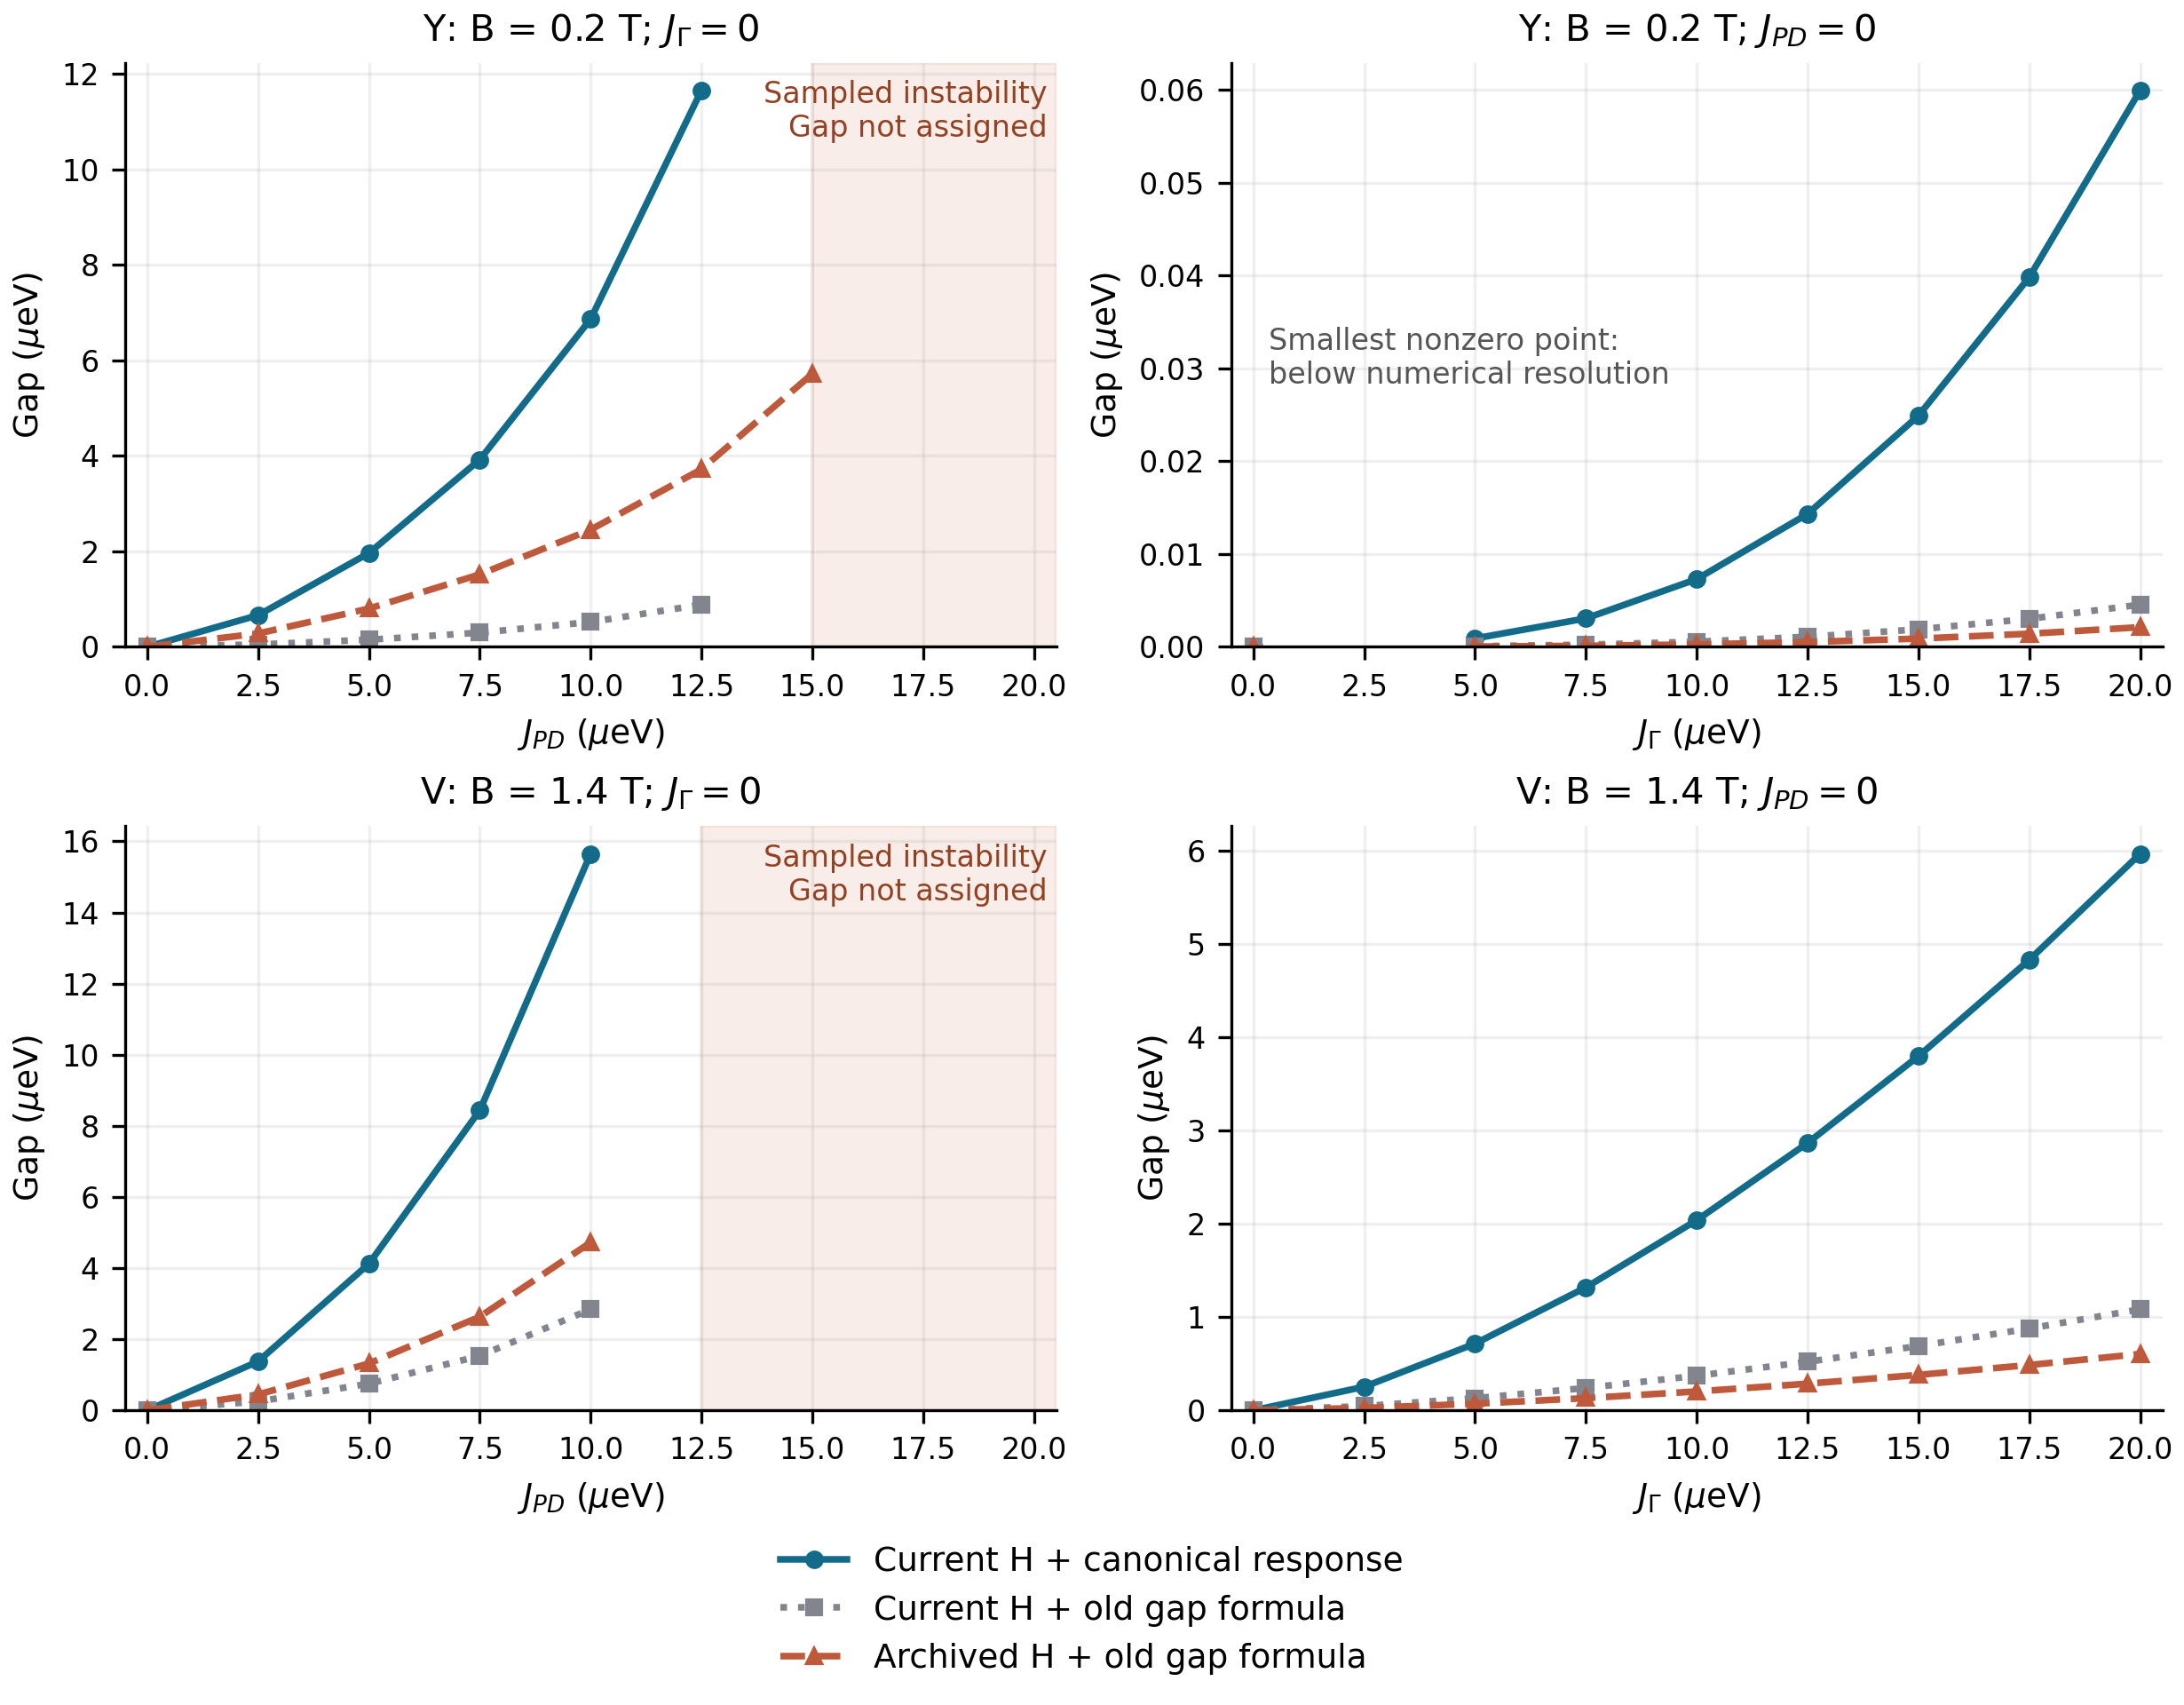
\includegraphics[keepaspectratio]{../../data-space/verification/260912-pseudo-goldstone/yv-pseudo-gap-comparison.png}}

}

\caption{\label{fig-yv-gap}Pseudo-Goldstone gap versus each SOC
coefficient. Blue: current Hamiltonian and canonical response. Gray:
current Hamiltonian and old formula. Orange: archived Hamiltonian and
old formula. Shading denotes instability detected in the sampled
current-Hamiltonian backgrounds; a physical gap is not assigned there.}

\end{figure}%

\subsubsection{Cross-checks of the canonical
response}\label{cross-checks-of-the-canonical-response}

The canonical response is cross-checked in both representative states
without recomputing the zero-point-energy curves. Explicit Y/V formulas
agree with the full \(A^{-1}\mathbf w\) response. Differentiating
independently relaxed field states at \(\delta h=10^{-5}\) meV gives
relative tangent errors below \(8.0\times10^{-9}\). Nonlinear
minimization at fixed magnetization approaches the derived tangent and
energy cost as the displacement decreases.

For all eight sign charts in each phase, a finite-difference Hessian of
the actual Cartesian bond energy agrees with the transformed analytic
Hessian within \(1.8\times10^{-9}\) meV; the relative susceptibility
change is below \(2.1\times10^{-8}\). The six-dimensional classical
tangent dynamics with a weak pinning potential reproduces both the gap
coefficient and the polar mode profile. Across pinning curvatures
\(10^{-7}\) and \(10^{-9}\) meV per cell, relative frequency and
mode-profile errors are below \(7.3\times10^{-8}\) and
\(2.6\times10^{-7}\), respectively.

These checks support the local classical reduction and its
normalization. They do not replace human physics review or provide an
independent one-loop self-energy calculation. Several checks share the
same classical energy or Hessian; their agreement is a consistency
check, not a wholly independent microscopic calculation.

\subsection{Approximation and interpretation}\label{sec-interpretation}

\subsubsection{Curvature order and coordinate
conventions}\label{curvature-order-and-coordinate-conventions}

In arXiv:1805.00947, Eqs.
(7)-(9)~\cite{rau2018}, the simple illustration uses equally weighted local transverse
coordinates. Its prefactor \(1/S\) belongs to that coordinate
normalization. Here the physical global azimuth has sublattice weights
\(\sin\vartheta_\alpha\), so one must compute the Berry coefficient or
use the magnetization coordinate directly.

Lin and Shi~\cite{lin2025} note that the curvature formula of
Ref.~\cite{rau2018} had been justified only for collinear order, and
that its derivation drops the nonlinear dependence of the rotation on
the soft angles, and with it a tadpole self-energy. They derive a
curvature formula for noncollinear order in which the angles are
normalized by the canonical commutator of the zero mode, not by equal
local weights. The Y and V states are noncollinear, so printing
Eq.~(1) of Ref.~\cite{rau2018} for them, as in Ref.~\cite{park2026},
lacks both ingredients. Equation~\eqref{eq-lswt-yv-pg-gap} supplies the
canonical normalization through \(\chi_z\), and takes \(C_\phi\) along
the exact rotated classical orbit, so the nonlinear part of the
rotation enters the curvature. Its correspondence with the type-I
expression of Ref.~\cite{lin2025} is structural; a term-by-term
comparison of the self-energy has not been made.

The leading type-I calculation does not require a quantum mixed
curvature to be identically zero. The classical energy is independent of
the common azimuth, so its mixed curvature vanishes. With the usual
expansion at fixed \(h/S\), the hard classical curvature is \(O(S^2)\)
and the quantum soft and mixed curvatures are \(O(S)\). The square of
the quantum mixed curvature is therefore subleading in the determinant
relative to the product of the classical hard and quantum soft
curvatures. Near additional soft directions that ordering can fail. Thus
setting the mixed term to zero is consistent with the present
leading-order reduction; it is not a separately demonstrated
leading-order error in the archived result.

The coordinate-relabeling check also needs a precise interpretation.
Under \(\vartheta_\alpha\mapsto-\vartheta_\alpha\),
\(\phi_\alpha\mapsto\phi_\alpha+\pi\) for selected sublattices, let
\(D_s\) be the diagonal sign matrix. The same physical response
transforms as \(A\mapsto D_sAD_s\), \(\mathbf w\mapsto D_s\mathbf w\)
and \(\mathbf x_*\mapsto D_s\mathbf x_*\), leaving \(\chi_z\) invariant.
Reusing the numerical vector \((1,1,1)\) in the new chart generally
chooses a different physical deformation. The old hard-curvature change
diagnoses an unspecified deformation rule, not a failure of the
classical energy's coordinate invariance.

\subsubsection{Validity checks}\label{sec-nbcp-gap-validity}

The checks below test the assumptions of
Eq.~\eqref{eq-lswt-yv-pg-gap} for \(J_{PD}\le0.010\) meV on the PD axis
and \(J_\Gamma=0.010\) meV on the \(\Gamma\) axis, with the uniform
sector at \(N=24\) and thermal sums at \(N=48\). The stability margin
also scans larger \(J_{PD}\).

\textbf{Orbit versus linear local coordinates.} Along the straight
tangent line of linear local coordinates, the parametrization of Rau et
al.~\cite{rau2018}, the background leaves the classical manifold at
second order. The zero-point curvature there is 13 to 35 times
\(C_\phi\) in the five Y and V cases checked. The excess equals the
zero-point gradient times the polar bending
\(\tfrac12\phi^2\sin\vartheta_\alpha\cos\vartheta_\alpha\) of the orbit
to \(2\times10^{-8}\) meV per spin. Adding the vacuum shift that this gradient
produces at order \(1/S\), through the classical third derivative,
restores \(C_\phi\) to within 0.1–0.4\%. This is the tadpole term of
Lin and Shi~\cite{lin2025}. Equation~\eqref{eq-lswt-yv-pg-gap} avoids it
by taking \(C_\phi\) along the exact orbit. Second derivatives of the
zero-point energy off the orbit are not used. They double with each
doubling of \(N\), because the gapless branch near \(\Gamma\) softens as
soon as the background leaves the classical manifold.

\textbf{Single-mode reduction.} The six-dimensional classical dynamics of
the uniform sector reproduces the \(\Gamma\)-point spin-wave frequencies
to \(2\times10^{-8}\) meV and has exactly one zero mode. With the
leading-order pinning \(C_\phi\) added along the orbit, its lowest
frequency equals \(\sqrt{C_\phi/\chi_z}\) to within 0.1\%, even for V at
\(J_{PD}=0.010\) meV, where the gap is 0.46 of the lowest hard
\(\Gamma\) mode.

\textbf{Stability margin.} The background at the selected angle stays
stable up to at least \(J_{PD}=0.014\) meV (Y) and 0.0115 meV (V). The
orbit fails first at the angular maxima \(\phi=\pi/6\bmod\pi/3\): for Y
at \(J_{PD}=0.014\) meV near \(|\mathbf k|\approx0.08\), and for V at
0.0115 meV near \(|\mathbf k|\approx0.19\). Above these couplings the
angular potential has no spin-wave value at its barriers, so neither the
harmonic fit nor the clock model applies, although the local gap at the
minimum is still defined. For V at \(J_{PD}=0.010\) meV the lowest
finite-momentum mode, 0.0144 meV, already lies below the uniform gap,
0.0156 meV, and the gap rises to 0.0232 meV at 0.0115 meV. These are
leading-order values close to an instability, where the next order is
expected to be large (inferred).

\textbf{V near \(r=1\).} The leading-order curvature
\(C_\phi=36\lambda_6(1-r^2)\) of Section~\ref{sec-nbcp-v-mixed-soc}
vanishes where each \(C_2'\mathcal T\)-symmetric minimum splits into two
minima related by \(C_2'\mathcal T\). The zero is therefore the soft mode
of a \(C_2'\mathcal T\)-breaking transition, not a failure of
Eq.~\eqref{eq-lswt-yv-pg-gap}. Higher orders shift where it occurs, and
near that point the leading-order value is not quantitative.

\textbf{Finite temperature.} At finite \(T\) the gap is set by the
curvature of the free energy~\cite{lin2025}. In the harmonic free energy
\(f=e_{\rm sw}+T\sum\ln(1-e^{-\omega/T})\) per spin along the exact
orbit, the ratio \(\Delta(T)/\Delta(0)=\sqrt{C_\phi(T)/C_\phi(0)}\) is
\begin{center}
\small
\begin{tabular}{@{}lcccc@{}}
\toprule
\(T\) (meV) & 0.0025 & 0.005 & 0.010 & 0.015\\
\midrule
Y, \(J_{PD}=0.010\) & 0.992 (0.998) & 0.951 (0.974) & 0.829 (0.893) & 0.802 (0.907)\\
V, \(J_{PD}=0.010\) & 0.996 (0.999) & 0.987 (0.997) & 1.037 (1.059) & 1.178 (1.208)\\
V, \(J_\Gamma=0.010\) & 1.000 (1.000) & 1.001 (1.000) & 1.020 (1.020) & 1.102 (1.102)\\
V, \(J_{PD}=0.010\), \(J_\Gamma=0.005\) & 1.060 (1.011) & 1.170 (1.059) & 1.392 (1.180) & 1.586 (1.294)\\
\bottomrule
\end{tabular}
\end{center}
Values in parentheses remove the lowest branch with
\(|\mathbf k|<0.25\) from the thermal sum. Those modes belong to the
phase field of the clock model, and the phase theory regenerates their
contribution through the angle dependence of its stiffness
(Section~\ref{sec-nbcp-matching-results}). The parenthesized values are
therefore the input for a phase theory that keeps \(\rho(\phi)\); the
unparenthesized values are the input for one with a constant stiffness.
Thermal fluctuations weaken the Y pinning and strengthen the V pinning.
In Y the change stays below 5\% up to 0.005 meV. These values assume a
locked angle and non-interacting magnons. The thermal correction to
\(\chi_z\) is of higher order in \(1/S\).

\textbf{Next order in \(1/S\).} The next order of \(\Delta^2\) needs
\(C_\phi\) at two loops, which requires interacting spin-wave vertices
not implemented here, and \(\chi_z\) at one loop. The latter is
\(-\partial_h^2e_{\rm sw}\) on the classical stationary state. It adds
\(+0.408\) to the classical \(\chi_z=1.111\) meV\(^{-1}\) per spin of
Y at 0.2 T (37\%), and \(+0.029\) to \(1.551\) of V at 1.4 T (2\%), at
\(J_{PD}=0.010\) meV. By itself the Y correction would lower the gap by
about 15\%. The two-loop \(C_\phi\) is unknown, so this is not a
next-order gap. The two-loop term of \(\chi_z\), from the nonlinear
spin-wave solver of the package roadmap
(\href{../../../data-space/verification/261003-nbcp-nonlinear-spin-waves/nbcp-nonlinear-spin-waves.json}{two-loop
check}, reproduced by
\href{../../../examples/nbcp_nonlinear_spin_waves.py}{the solver
example}), is \(-24\%\) of the classical
value for Y and \(-54\%\) for V; the V magnetization changes by
\(-0.040\) at one loop and \(-0.048\) at two loops. The V series is
therefore not controlled at 1.4 T, where V lies close to its classical
stability edge; soft modes there are the likely cause (inferred). The
leading Y gap carries a next-order uncertainty of tens of percent. The
relation \(\Delta^2=C_\phi/\chi_z\) itself holds only at leading order
in \(1/S\), so the next-order gap needs a separate two-loop dynamical
calculation, which has not been done.

\subsubsection{Limits of the comparison}\label{limits-of-the-comparison}

This verifies the classical orbit, current quadratic Hamiltonian
coefficients, canonical normalization and numerical curvature
calculation. It is not an independent full one-loop self-energy
calculation, an all-orders prediction for S=1/2, or proof of global
phase stability. The finite-temperature gaps of
Section~\ref{sec-nbcp-gap-validity} are harmonic estimates. The
field-induced internal XXZ branch and the zero-field internal
pseudo-Goldstone mode are different modes and are not plotted here.

The shaded portions of the gap plots indicate sampled unstable spin-wave
backgrounds. Missing weak-Gamma Y points indicate inadequate numerical
resolution. Neither is assigned a physical zero gap. The finite-mesh
minimum magnon frequency is recorded as a diagnostic and is never used
as the pseudo-Goldstone gap.

A comparison with the published Figure 4 is conditional on the
parameters and available local code. The exact source revision and
numerical data used for the published gap curve have not been
established.
